\section{CP model}


\subsection{Decision variables}

The CP model relies on the following decision variables:
\begin{itemize}
    \item For each package $p$, $A_p \in [1, m]$ (\texttt{assignments[p]} in MiniZinc) indicates which courier delivers it. More specifically, $A_p = c$ iff the package $p$ is delivered by the courier $c$.
    
    \item For each courier $c$, $P_{c, d}$ (\texttt{path[c, d]} in MiniZinc) is defined following \Cref{eq:path_def}.
\end{itemize}



\subsection{Objective function}
Once the route of each courier has been found, the objective function is computed as follows:
\begin{equation}
    \max_{c \in [1, m]} \sum_{\substack{d \in [1, n+1]:\\P_{c, d} \neq d}} D_{d, P_{c, d}}
\end{equation}


\subsection{Constraints}

To respect the capacity limit of each courier, the following constraint can be defined:
\begin{equation}
    \forall c \in [1, m]: \sum_{p \in [1, n]: A_p = c} s_p \leq l_c 
\end{equation}
In MiniZinc, the global constraint \texttt{bin\_packing\_capa} also models this. In our experiments, we did not notice significant differences between the two formulations and decided to use the latter following the best practice of preferring global constraints.

To model the route, the following constraints have to be imposed:
\begin{equation}
    \label{eq:cp_constr_route_depot}
    \forall c \in [1, m]: 
    \begin{cases}
        P_{c, n+1} = n+1    & \text{if $\nexists p \in [1, n]: A_p = c$} \\ 
        P_{c, n+1} \neq n+1 & \text{if $\exists p \in [1, n]: A_p = c$} 
    \end{cases}
\end{equation}

\begin{equation}
    \label{eq:cp_constr_route_packs}
    \forall c \in [1, m],
    \forall p \in [1, n]: 
    \begin{cases}
        P_{c, p} = p    & \text{if $A_p \neq c$} \\
        P_{c, p} \neq p & \text{if $A_p = c$} 
    \end{cases}
\end{equation}

The constraint defined in \Cref{eq:cp_constr_route_depot} imposes that, for each courier, the depot has a successor only if that courier delivers at least a package. On the same note, \Cref{eq:cp_constr_route_packs} imposes that only the packages delivered by a specific courier have a successor in the route.
Moreover, it is necessary to impose that the route defined by $P_c$ is a Hamiltonian cycle that passes through the relevant destinations. In MiniZinc, this can be easily modelled by using the global constraint \texttt{subcircuit}.


\subsubsection{Symmetry breaking constraints}

For CP, we experimented with both symmetry breaking constraints defined in \Cref{eq:cp_symm_amount,eq:cp_symm_packs}. Moreover, we experimented with a stronger version of these constraints that is applied between two couriers whose actual loads are interchangeable. This is defined by the following condition:
\begin{equation}
    \label{eq:cp_symm_strong}
    \max\left\{ L_{c_1}, L_{c_2} \right\} \leq \min\left\{ l_{c_1}, l_{c_2} \right\}
\end{equation}
where $L_c$ is the actual load carried by the courier $c$.



\subsection{Validation}

\subsubsection{Experimental design}

We experimented variations of our models using as solvers Gecode, Chuffed, and OR-Tools. The search order for all models assigns the packages (\texttt{assignments}) first and then searches for the route (\texttt{path}) of each courier in decreasing order of capacity. Regarding search, we experimented several combinations of variable selection and assignment strategies on a subset of instances and only used the best ones to obtain the final complete results.


\subsubsection{Experimental results}

From some preliminary experiments, we observed that first fail and largest domain with weighted degree (\texttt{dom\_w\_deg}) are the best performing search strategies. Therefore, we performed the full experiments using as search strategy \texttt{dom\_w\_deg} for \texttt{assignments} and \texttt{first\_fail} for \texttt{path}, respectively. Moreover, between the two symmetry breaking constraints, we observed that the lexicographic ordering defined in \Cref{eq:cp_symm_packs} has better performances and therefore present only those results. The objective values found by the most significant models are reported in \Cref{tab:cp_results}.

\begin{table}[ht]
    \caption{Selected subset of CP results. Results in \textbf{bold} are solved to optimality. Instances that are all solved to optimality have been omitted.}
    \label{tab:cp_results}
    \centerline{
        \begin{tabular}{c|cccccccccccc}
            \toprule
            & \multicolumn{6}{c}{Gecode} & \multicolumn{3}{c}{Chuffed} & \multicolumn{3}{c}{OR-Tools} \\
            \\[-3ex] % Remove vertical line gap
            \cmidrule(lr){2-7} \cmidrule(lr){8-10} \cmidrule(lr){11-13}
            Id & \rot{plain}    & \rot{luby}    & \rot{lns80}   & \rot{lns95}   & \rot{\makecell[l]{lns95\\[-0.3em]\small+ SB \eqref{eq:cp_symm_packs}}} & \rot{\makecell[l]{lns95\\[-0.3em]\small+ SB \eqref{eq:cp_symm_packs}\eqref{eq:cp_symm_strong}}} & \rot{plain} & \rot{luby} & \rot{SB \eqref{eq:cp_symm_packs}} & \rot{plain} & \rot{\makecell[l]{plain\\[-0.3em]\small+ FS}} & \rot{\makecell[l]{SB \eqref{eq:cp_symm_packs}\\[-0.3em]\small+ FS}} \\ 
            \midrule
            7  & 201            & \textbf{167}  & \textbf{167}  & \textbf{167}  & \textbf{167}  & \textbf{167}  & \textbf{167}  & \textbf{167}  & \textbf{167}  & 408           & \textbf{167}  & \textbf{167}  \\ 
            9  & \textbf{436}   & \textbf{436}  & \textbf{436}  & \textbf{436}  & \textbf{436}  & \textbf{436}  & \textbf{436}  & \textbf{436}  & \textbf{436}  & 617           & \textbf{436}  & \textbf{436}  \\ 
            11 & 594            & 597           & 528           & 490           & 503           & --            & 963           & --            & 756           & 1669          & 1189          & 1081          \\ 
            12 & 449            & 428           & 375           & \textbf{346}  & 348           & --            & 833           & 1061          & 785           & 1605          & 706           & 899           \\ 
            13 & 648            & 704           & 656           & 616           & 610           & 624           & 1126          & 914           & 1126          & 1734          & 584           & 746           \\ 
            14 & 725            & 972           & 794           & 715           & 792           & --            & 1449          & --            & 1089          & --            & --            & --            \\ 
            15 & 659            & 901           & 765           & 738           & 803           & --            & 1292          & --            & --            & --            & --            & --            \\ 
            16 & 451            & 294           & \textbf{286}  & \textbf{286}  & \textbf{286}  & --            & 487           & 636           & 694           & 998           & 467           & 363           \\ 
            17 & 1324           & 1468          & 1119          & 1076          & 1155          & --            & --            & --            & --            & --            & --            & --            \\ 
            18 & 691            & 806           & 675           & 662           & 620           & --            & 1321          & --            & 1779          & --            & --            & --            \\ 
            19 & 554            & 412           & 336           & \textbf{334}  & \textbf{334}  & --            & 795           & 1079          & 765           & 1521          & 623           & 577           \\ 
            20 & 1139           & 1369          & 1104          & 1068          & 1075          & --            & --            & --            & --            & --            & --            & --            \\ 
            21 & 779            & 687           & 600           & 516           & 529           & --            & 2104          & 2140          & 993           & 2115          & 1226          & --            \\ 
            \bottomrule
        \end{tabular}
    }
\end{table}

For Gecode, we experimented different search approaches by testing restart methods, large neighborhood search (LNS), and varying symmetry breaking constraints. We observed that, compared to a depth-first approach, by simply restarting search following the Luby sequence there is a mixed impact on the results with both positive and negative effects. Instead, by also using LNS, results tend to improve globally and we observed that a higher retain probability, with a peak at around $95\%$, works better. Regarding symmetry breaking constraints, we observed that they tend to worsen the final objective value in the majority of the cases, most reasonably due to the fact that the overhead to impose them is higher than the speed-up in search. For a visual comparison, we show in \Cref{fig:cp_obj_plots} the evolution of the objective value during search. It can be seen that without restart the objective stops improving in the early stages of search as it most likely gets ``stuck" in a branch of the search tree. By introducing some non-determinism, the objective reaches lower values, with LNS being the fastest and best performing.

\begin{figure}[H]
    \centering
    \begin{subfigure}{0.49\linewidth}
        \centering
        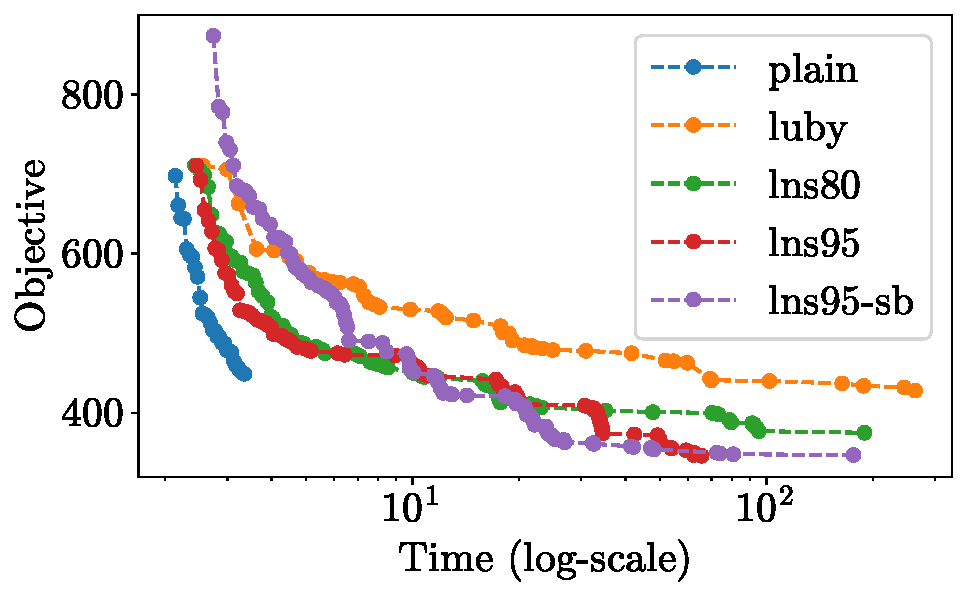
\includegraphics[width=\linewidth]{img/cp/obj-plot_inst12.pdf}
        \caption{Instance 12}
    \end{subfigure}
    \hfill
    \begin{subfigure}{0.49\linewidth}
        \centering
        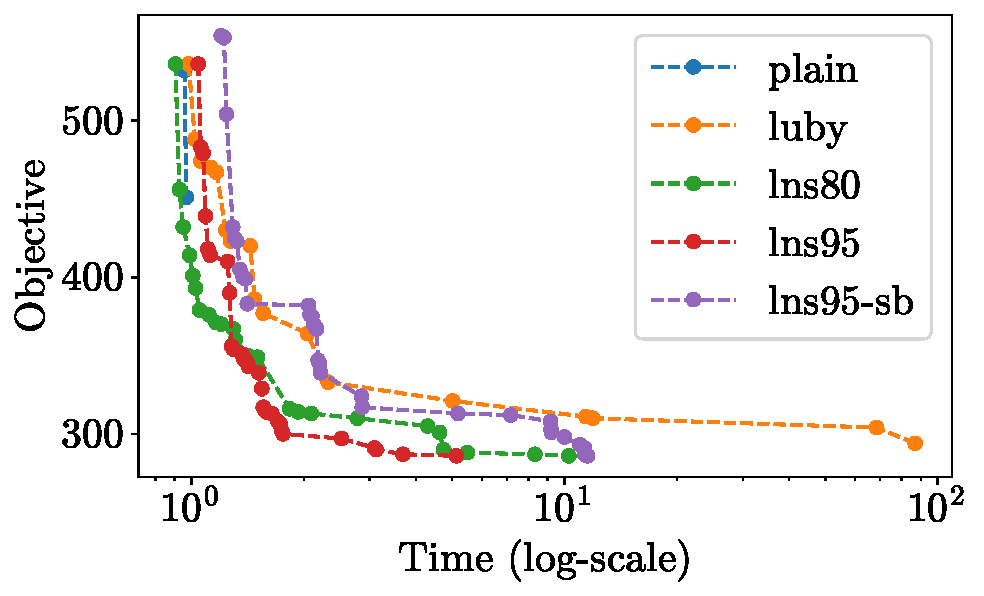
\includegraphics[width=\linewidth]{img/cp/obj-plot_inst16.pdf}
        \caption{Instance 16}
    \end{subfigure}
    \caption{Intermediate solutions using Gecode}
    \label{fig:cp_obj_plots}
\end{figure}

For Chuffed, we only experimented with restarts and symmetry breaking constraints as LNS is not available through MiniZinc. Moreover, as indicated in the documentation\footnote{\url{https://docs.minizinc.dev/en/stable/solvers.html}}, we tried enabling free search mode but only obtained worse results. Compared to Gecode, results on bigger instances are generally all worse, while smaller instances tend to be solved faster by Chuffed. As in Gecode, restarts, which we only experimented with random variable selection as it is the only non-deterministic search strategy available, and symmetry breaking constraints both yield mixed effects on the final result.

Finally, for OR-Tools, we conducted fewer experiments as it supports fewer MiniZinc annotations. In this case, we observed that enabling free search mode allows obtaining better results and, similarly to Gecode and Chuffed, symmetry breaking constraints have mixed results. As a side note, we must also observe that, as suggested in the documentation, these results are worse as OR-Tools performs better with multi-threading. 

